\documentclass[12pt,a4paper,stu, donotrepeattitle, floatsintext]{apa7}


\usepackage[utf8x]{inputenc}
\usepackage{amsmath}
\usepackage{graphicx}
\usepackage{mathptmx}
\usepackage{scrextend}

\usepackage[english, russian]{babel}

\linespread{2}
\usepackage[colorinlistoftodos]{todonotes}

\usepackage{apacite}

\title{\large{How Does School Schedule Affect Eleventh Grade Students in Nazarbayev Intellectual School of Physics and Mathematics in Nur-Sultan?}}
\author{Yernur Kairollayev}
\affiliation{Nazarbayev Intellectual School of Physics and Mathematics}
\course{Global Perspectives and Project Work \\ Grade 11D1}
\professor{Teacher R.J.}
\duedate{13 May 2022}

\begin{document}
\maketitle
\section{Introduction}
As an eleven-grade student of Nazarbayev Intellectual school of Physics and Mathematics in Astana (here and after 11 grader) I had noticed that I am exhausted after the school and cannot perform as productive as during the school day. After brief discussion with my peers, we all agreed that we feel tired in the beginning of the school day and in the evenings. 11 graders’ lessons start at 8AM and finish at 4 PM. After brief research in the YouTube platform, I have found a video called "Is your school slowly destroying your brain?" \cite{youtube} based on a "Why we sleep: Unlocking the Power of Sleep and Dreams" \cite{Walker2017}, which states that adolescents naturally go to bed later and get up later than adults. Despite the later start time comparing with American students, 11 graders still need to get up early in order to commute to school using public or private means of transportation, unlike students from the United States of America with famous school buses. Which means that debate about effects of the timetable on their productivity is open.

Considering scientific lens, one research states that in the early morning, productivity of school students is at its maximum, and falls during the day \cite[p. 10]{Pope2016}. Which means that early start of the classes at NIS PhM is beneficial for students, as they spend more time learning while they have higher level of productivity. Which is crucial to achieve satisfying academical performance.

On the other hand, group of researchers state that students during classes, which start early performing worse. In addition to that, they have lower productivity during subsequent classes, than their peers without classes, which start early in the morning \cite{Carell2018}. Authors also provide causes of these results, namely, circadian rhythms of adolescents which are switched a bit later than the school starts (p. 18).  This means, that NIS PhM in Astana students have lower productivity during school day, which may lead to academical problems.

The importance of the research on this topic cannot be undermined, as students’ productivity affects their results and academical outcome. It is especially important to get quality education for NIS students, as they get enormous grants, in comparison with municipal schools’ students, from the republican funding \cite{Massimov_res, zakon_2020}.

The purpose of the research is to access effects of the schedule of 11 graders in NIS PhM in Nur-Sultan on their productivity and performance. 

I claim that the schedule of 11 graders in NIS PhM in Nur-Sultan is negatively affecting their productivity during school day, due to sleep schedule disruptions and distortion of circadian rhythms.

\newpage
\section{Aims}

High school is an important part of a person’s life, as it is time, when people prepare for a university and any other future path. Which is why it is crucial to stay productive in order to get high quality education and preparation. However, there is no research, evaluating effects of NIS schedule on 11 graders.

The goal of this research is to evaluate effects of school’s start time, end time and on 11 graders, and their productivity’s dependency on time considering biological development of adolescents.

As the research goes, I will try to answer these questions:

\begin{itemize}
    \item How does school start time affect 11 graders’ productivity?
    \item How do circadian rhythms affect 11 graders’ productivity?
    \item How do 11 graders’ productivity depend on time?
\end{itemize}

In order to answer aforementioned questions, I will analyze secondary sources, namely research conducted on this topic. They will help me to gain experience from other countries and create basis for a scientific, especially biological, lens. Also, I will conduct and interview with an unbiased 11 grader, who can tell more about their thoughts on the timetable.

Different aspects of the school timetable are likely to differently affect students’ productivity. There may be advantages and disadvantages for an early start time and long duration of the school day, I do not expect anything about the first yet, however I am expecting more negative sides of prolonging school days.

\section {Context}

The first thing important to look for is evidence of better health and lower sleepiness with later start of school day. There is a study on this matter called “Impact of Delaying School Start Time on Adolescent Sleep, Mood, and Behavior” \cite{Owens2010}. It was looking into effects of 30 minutes delay of an independent school start time from 8 AM to 8:30 AM (p.2) via 2 surveys of students before the intervention and after. The results of their research have shown, that mean amount of sleep students get during nights after the school increased from 7-7.9 to 8-8.9 (p.4). Also, lower number of students reported sleepiness related behavior, but still most of participants were struggling to do homework due to weariness and to get up early and stay awake (Figure 1) (p. 5). As one can see, delay of 30 minutes reduces all of problems, however some of them still are high enough. Ergo, later start of the school benefits health of 11 graders.

\begin{figure}[H]
    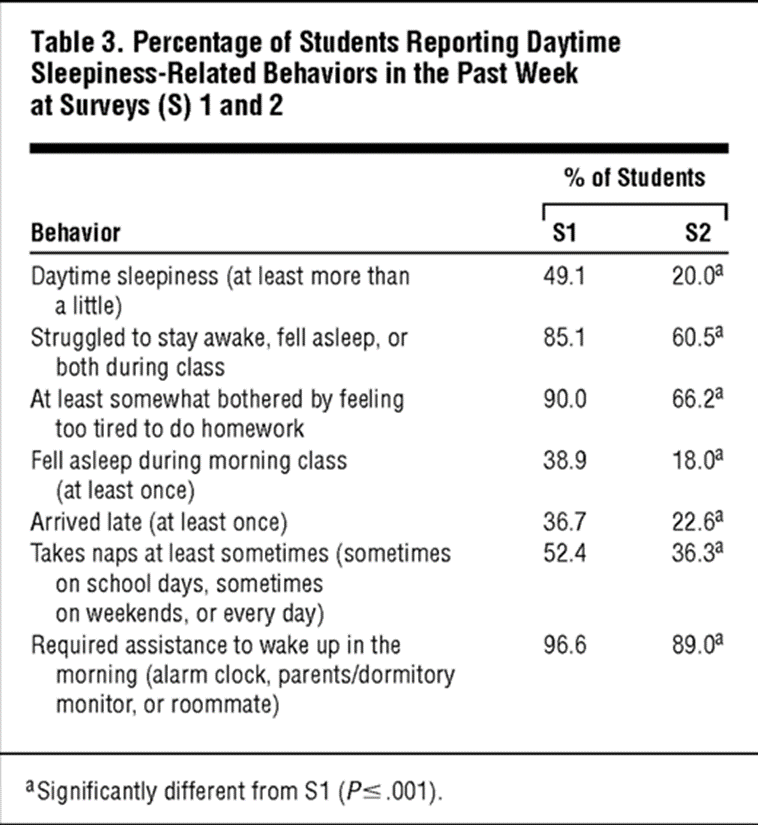
\includegraphics{picture1.png}
    \centering
    
    {Figure 1. \cite{Owens2010}}
\end{figure}

Moreover, there is evidence, that 9 in the morning is still early to start the school. Another research “Is 8:30 a.m. still too early to start school? A 10:00 a.m. school start time improves health and performance of students aged 13-16” \cite{Kelley2017} conducted a three-year experiment, where they started observation from the year 0 with start time at 8:30 a.m. and then 2 years with start time at 10 a.m. and then in year three they returned to start time at 8:30 a.m. Results have shown, that intervention to the schedule led to lower rates of absences due illness and better academic achievements. After getting back to the original school start time, improvements have been kept. This research can be used because there was no significant difference among different ages in the research 30 minutes delay to 8:30 a.m. \cite{Owens2010}, hence it can be concluded that school schedule still has negative impact on productivity and health of 11 graders.

There is particular research on sleep distortion and its connection to productivity, called “Being physically active increases yet sedentary bouts and lack of sleep decrease work ability” \cite{Giurgiu2021}. Researchers used 3 accelerometers on each person as a complex system which collects data of all kinds of movements (p. 2-3). Results mainly were analyzed on sedentary behavior; however, sleep patterns were analyzed too. Deviation from normal amount of sleep (approximately) resulted in worse productivity (p.7). Which means early start of the school slightly decreases productivity of 11 graders.

One of the proposed reasons of productivity drivers is that circadian rhythms affect mind of people and their distortion \cite{Carell2018}. That is why it is necessary to find evidence that adolescents have delay in daily circadian cycle. A team of scientist made research on this particular topic, called “Sleep, circadian rhythms, and delayed phase in adolescence” \cite{CROWLEY2007602}. It is based on surveys of students 11 to 19 years old, finding a significant gap between bedtime and risetime on weekday and weekends (p.2). Results have shown, that delayed circadian phase in adolescents is due to both external and internal (biological and homeostatic) factors (p.8). Using their research in can be shown, that first lesson of 11 graders is during the time, when they are usually asleep during weekends.

As the mornings in winter are darker than in the summer, and the school start time doesn’t change in the winter, leading to the darker classrooms during first two lessons, and  light and dark affect circadian rhythms also circadian rhythms affect sleep \cite{nigms}, it is important to search for evidence of light changes disrupting sleep and school performance. There is a research, conducting experiment on circadian light exposure, called “Measuring circadian light and its impact on adolescents” \cite{Figueiro2011}. They used orange glasses to block the circadian light from one group of students. They and the control group studied in same conditions for one week wearing daysimeters to find changes between daylight exposure and circadian timing. As a result, it was concluded that lower daylight exposure leads to later circadian timing. Despite this fact connections between scholastic performance and daylight exposure were inconclusive and have shown low correlation (p.12). This means, that the distortion of circadian rhythms is not the reason of changes in performance and attendance levels in research and 11 graders’ productivity is not affected by circadian rhythms \cite{Kelley2017, Owens2010}. However, this doesn’t change the fact that they are studying during low circadian phase, as shown in previous paragraph.

\section{Method}
The research design contains secondary research and will contain primary research. The first is needed to obtain background information and identify the situation concerning research questions. The second will be made to gather qualitive data about the situation of 11 graders via interview.

The background information was collected via Internet libraries because library in the NIS PhM in Astana and other local libraries did not provide current information on the research topic and didn’t have printed volumes of journals. I used Google Scholar and ProQuest online databases as they mostly contain credible sources, namely works of researchers such as books and journal articles. To be sure in their credibility, I checked authors, places of publication and their bias.

The primary research method will be is an interview with an average female 11 grader. I decided to choose her to get more data with a personal opinion, which could open the way for more research on this topic across the country. To do the interview I will use audio recorder in order to store the interview and I will personally transcribe the interview. The whole transcription will be attached to the appendices of the paper.

One more crucial thing to do is data triangulation, which will help to increase the validity and credibility of my sources. In particular, it will help me to benefit results of the future interview and survey with my secondary sources. Generally, it will increase credibility of my research paper with results closer to the reality and reliability of my research paper.

\section{Results and conclusion}

The interviewee was definite in her answers. She is an early riser, but due to amount of homework, she has sleep deprivation (only 6 hours of sleep on weekdays). Which is extremely harmful, as found in researches (2003) \cite{Giurgiu2021,dongen2003} Due to formed routine, it was hard for her to switch to a normal schedule with start of lessons at 8 AM, also it led to less sleep due to longer school days. And introduced large number of 20-minute brakes interrupts her productivity. But most importantly, she self-reported that she had better productivity, when school started at 9 AM, which corresponds with current scientific consensus, made on research \cite{Kelley201,Owens2010}. Also, her self-reported productivity does not correlate with circadian rhythms \cite{Figueiro2011}. Unexpectedly interviewee prefers to learn at home rather than in school, as it is more producitve and comprehensive this way.

\textit{How does school start time affect 11 graders’ productivity?}

Both primary and secondary \cite{Kelley2017, Owens2010} research have shown, that later start time of the school is beneficial. As start time is one of the essential parts of the schedule, these conclusions should not be ignored.

\textit{How do circadian rhythms affect 11 graders’ productivity?}

Both primary and secondary \cite{Figueiro2011} research have shown that productivity circadian rhythm cannot be considered as a productivity driver. Thus, schedule managers should not consult with biologists.

\textit{How do 11 graders’ productivity depend on time?}

This is only slightly covered question. Primary research has shown that there is time dependence of productivity due to fatigue. However direct connection wasn’t found. Importance of this topic cannot be denied as schedule is a way to organize time.

\section{Limitations}
The hardest limitation of my research was the time limit. Due to inability to do research for 3 weeks straight, I had to quickly do the primary research, which may have affected its quality. However, I did my best to conduct beneficial interview and qualitatively analyze it. Also because of that, I had to give up on idea of conducting a survey, which would be highly beneficial, considering my research questions. Instead, I used interview, which was the second-best option for my research.
	
Due to small amount of time, I could not find the room for an interview during weekends, which is why I held it via audiochat. There were some background noises on either side, so I had to manually transcribe the audio recording. Also, due to different language of the interview I had to translate it to make it understandable for the main auditory. Unfortunately, meaning or tone of some phrases could be lost due to translation. However, I did my best doing that, so almost all of the mood of the interview is not lost. 

I interviewed only one person, so making conclusions basing only on her answer is quite dangerous, because it is uncheckable that her answer is not an outlier. However, I used general questions, because they offer ability to know her opinion on other people, because some of it is leaked or told during the brake.
	
Moreover, online libraries lacked big number of free qualitative and quantitative researches on the topic, which led me to using the limited secondary sources. This could mean that this topic is not satisfyingly comprehended by secondary research.

\section{Evaluation}
Overall, the research was quite productive, and has enough evidence to raise a concern about efficiency and safety of the current timetable at NIS PhM in Astana. As far as I am concerned, each section of the research has been conducted properly, however, due to my lack of expertise, and experience, and other aforementioned limitations, there are still some things that can be improved.	

The secondary research was conducted with persistence but due to limited amount of free literature it could be incomprehensive. However, all of the found were thoroughly analyzed and all of the related parts were used to their maximum. All of three research questions were comprehended and discussed in the secondary research. The secondary research can be improved with more time on it and usage of other online libraries; however it would have much effect as all of the aforementioned papers were almost everything that Google Scholars database and search engine could find on the topic.

The main interview was conducted poorly due to lack of time. This led to its longer duration. However, all of the 3 research questions were fully covered in the course of it. Also, during the thematic analysis gaps were found, that is why follow-up interview had to be conducted. Second interview was conducted better due to more experience and greater confidence in myself and in my interviewee, as the procedure was quite familiar, and was conducted in real life, instead of online call. After that interview was comprehensive enough to finish the thematic analysis. The interview could be improved with a more thorough analysis and conducting focus-group interview. Generally, primary research can be improved with the survey and interview with expert basing on secondary sources and survey.

The research was quite affective on my perspective on the topic. In the beginning I thought that a) sleep deficiency is harmful for adolescents; b) earlier start of the school is effective c) students productivity depends on circadian rhythms, therefore it is time dependent. After the research I have come to the conclusion, that perspective a) was correct, b) was incorrect c) was partially incorrect, as productivity doesn’t depend on circadian rhythms, however, is directly depend on weariness of a student. Also unpredicted themes were raised, such as difference between covering the program at home and at school, efficiency of lessons, resting at school. This means, that there are still branches to be researched.

\newpage
\section{Further research}

The outcome of the research suggests a further area to study.
	
Firstly, the efficiency of school program should be evaluated. Some topics could be covered too broadly and others too shortly. In the 11th grade students are quite capable of learning school material at home, as interview has shown. Along with it, efficiency of lessons should be judged and analyzed. Probably there are better ways to conduct lessons. Qualitative research with a quite broad focus group could prove efficient as it allows to collect reactions and response of students.
	
Secondly, the efficiency of school schedule was evaluated considering 11 graders. Meaning, that timetable of other grades and their response should be evaluated and the teachers’ response to the timetable should be evaluated, as they are too, very important part of the studying process. For this purposes, quantitative research could prove efficient as results can be used in planning the schedule and timetable.

\newpage

\bibliographystyle{apacite}
\bibliography{reference.bib}

\newpage
\section{\textbf{Appendix A. Main Interview Transcript}}

Topic: \textbf{How Does School Schedule Affect Eleventh Grade Students in Nazarbayev Intellectual School of Physics and Mathematics in Nur-Sultan?
Transcript of the interview: Interviewer (\textbf{Yernur}), Interviewee (Adel)}
Time of the interview: 20:00 on Sunday

\textbf{Yernur}: 

Добрый день, сейчас мы начнем интервью, и начнем с вопроса ты сова или жаворонок?

Good afternoon, now we will start the interview, and we will start with the question are you an owl or an early riser?

Adel:

Я лично жаворонок

I am personally an early riser

\textbf{Yernur}:

Хорошо, и во сколько ты просыпаешься в школьные дни?

Okay, and what time do you wake up on school days?

Adel:

Обычно, в 6 утра

Usually, at 6 am

\textbf{Yernur}: 

В 6 утра, хорошо, и насколько сложно или просто?

At 6 am, ok, and how difficult or simple is it?

\textbf{\textit{Adel}}

Это довольно тяжело, потому что обычно я ложусь в 12 ночи, и просыпаюсь в 6. И поэтому 6 часов сна не хватает

It's pretty hard because I usually go to bed at 12 at night and wake up at 6. And that's why 6 hours of sleep is not enough

\textbf{Yernur}:

Насколько тебе сложно просыпаться в выходные?

How hard is it for you to wake up on the weekend?

\textbf{\textit{Adel}}

Ааа, бывает тяжело, потому что нету и необязательно вставать очень рано, но я стараюсь вставать хотя бы до 10 

Aah, it can be hard, because there is no need to get up very early, but I try to get up at least before 10

\textbf{Yernur}: 

Ясно, давай перейдём на твоё самочувствие в будние дни. Как ты себя чувствуешь на первом уроке? (Может сонной, не можешь сконцентрироваться, или энергичной, или может быть даже головные боли есть?)

Okay, let's move on to how you feel on weekdays. How do you feel in the first lesson? (Maybe sleepy, can't concentrate, or energetic, or maybe even have headaches?)

Adel:

Ну на первых уроках я в основном более сконцентрированная и могу как-бы… голова работает лучше, и мне кажется на первых уроках

Well, in the first lessons I'm mostly more concentrated and I can sort of... my head works better, and it seems to me in the first lessons

\textbf{Yernur}: 

Ясно, а на уроках которые идут после первого и до обеда.

Okay, and on the lessons that go after the first and before lunch.

Adel:

Ну в принципе так же, но ближе к обеду уже начинаешь уставать от количества уроков и нагрузки, поэтому там уже больше усталость 

Well, basically the same, but closer to lunch you already start to get tired of the number of lessons and the load, so there is more fatigue

\textbf{Yernur}: 

Ясно, а в послеобеденные уроки?

Okay, but in the afternoon lessons?

\textbf{\textit{Adel}}

На послеобеденных уроках уже тяжелее, потому что уже проходит 10 уроков и очень сильно тяжело сосредоточиться на уроке, на учителе и в принципе делать какую-то работу

It's harder in the afternoon lessons, because 10 lessons are already taking place and it's very hard to focus on the lesson, on the teacher and, in principle, to do some work

\textbf{Yernur}: 

Ага, хорошо, и как ты себя чувствуешь себя после школы, какая у тебя продуктивность после школы при выполнении домашнего задания?

Yeah, well, and how do you feel after school, what is your productivity after school when doing homework?

\textbf{\textit{Adel}}

В основном после школы я не могу нормально делать домашнее задание, потому что после 10 или обычно 8 уроков, я уже сильно устаю и предпочитаю поспать и делать это ближе к 12, либо делать рано утром, встать пораньше чем в 6 утра

Basically, after school, I can't do my homework properly, because after 10 or usually 8 lessons, I'm already very tired and prefer to sleep and do it closer to 12, or do it early in the morning, get up earlier than 6 in the morning

\textbf{Yernur}: 

Хорошо, понятно. Давай теперь поговорим о расписании в целом. Насколько сложно было перейти с расписания, которое ввели из-за эпидемиологической ситуации, то есть когда мы приходили в 9 утра, на нормальное расписание, когда мы начали приходить в 8 утра?

Okay, I see. Now let's talk about the schedule in general. How difficult was it to switch from the schedule that was introduced due to the epidemiological situation, that is, when we came at 9 a.m., to the normal schedule when we started coming at 8 a.m.?

Adel:

Аа, ну было тяжело, потому что как-бы, когда уроки начинались в 9 утра, у меня был один распорядок дня и у меня было больше времени на утренние процедуры, и была возможность делать уроки с утра. А, потом когда уроки переставили на 8 утра, пришлось вставать ещё раньше, но также у нас увеличилось количество времени, которое мы проводим в школе, поэтому и нагрузка прибавилась, поэтому я ложилась так же и вставала ещё раньше

Ah, well, it was hard, because, as it were, when lessons started at 9 in the morning, I had one daily routine and I had more time for morning procedures, and I had the opportunity to do lessons in the morning. And then, when the lessons were moved to 8 a.m., I had to get up even earlier, but we also increased the amount of time we spend at school, so the load increased, so I went to bed the same way and got up even earlier

\textbf{Yernur}:

Ага, и получается, какое расписание ты предпочитаешь? Первое или второе?

Yeah, and, which schedule do you prefer? The first or the second?

\textbf{\textit{Adel}}

Лично я предпочитаю первое

Personally, I prefer the fisrt

\textbf{Yernur}: 

Ага, и почему?

Yeah, and why?

\textbf{\textit{Adel}}

Потому что, ну во первых есть больше времени с утра, и необязательно вставать очень рано, и есть время чтобы выспаться, и набраться своих сил [inaudiable]. А также в новом расписании есть очень много больших перемен, которые по моему мнению занимают слишком много времени, которое можно было бы потратить на школьные занятия или тот же самые отдых?

Because, well, first of all, there is more time in the morning, and it is not necessary to get up very early, and there is time to sleep and gain your strength [inaudible]. And also there are a lot of big changes in the new schedule, which in my opinion take too much time, which could be spent on school classes or the same rest?

\textbf{Yernur}:

Получается, когда было ощущение большей продуктивности?

Wthere was a feeling of greater productivity?

\textbf{\textit{Adel}}

Эм, в старом расписании, когда начиналось в 9

Um, in the old schedule, when it started at 9

\textbf{Yernur}: 

Кроме того, что уроки начали начинаться в 8 утра, у нас добавились 4 дополнительные перемены по 20 минут. Как они влияют на твою продуктивность и концентрацию?

In addition to the fact that lessons started starting at 8 am, we have added 4 additional breaks of 20 minutes each. How do they affect your productivity and concentration?

\textbf{\textit{Adel}}

Я бы сказала негативно, средне то есть, а потому что, наверное в первой половине дня 20-минутные перемены, будут время немножко отдохнуть, перевести дух, и правда помогают. Однако уже после обеда одна перемена 20-минутная, о которой… одна или две, на которых честно говоря уже не знаешь что делать. И [inaudiable] недосыпаешь, либо уже теряешь концентрацию на уроках, и если вообще перемена стоит между двумя уроками, между одним уроком математики и вторым уроком математики, то потом уже тяжело вернуться в процесс урока и понять.

I would say negatively… I mean neutrally, but because, probably, in the first half of the day there is one 20-minute brake, there will be time to rest a little, take a breath, and they really help. However, after lunch there is one 20-minute break, about which... one or two, on which, to be honest, you no longer know what to do. And [inaudible] you don't get enough sleep, or you lose concentration in lessons, and if there is a change at all between two lessons, between one math lesson and the second math lesson, then it's hard to go back to the lesson process and understand.

\textbf{Yernur}: 

Интересно, так, и… сейчас секунду, как по вашему, какие ещё факторы, кроме этих 20-минутных перемен и начала уроков в 8 влияют на продуктивность учеников и лично на твою продуктивность.

It's interesting, so, and... one second, in your opinion, what other factors besides these 20-minute changes and the beginning of lessons at 8 affect the productivity of students and your productivity personally.

\textbf{\textit{Adel}}

Наверное, я бы сказала количество уроков в день, потому что слишком большое количество уроков [разрыв связи] 

I would probably say the number of lessons per day, because there are too many lessons [disconnection]

\textbf{Yernur}: 

Извиняюсь, пока ты отвечала, связь немного прервалась, можешь пожалуйста ещё раз повторить?

I'm sorry, while you were answering, the connection was interrupted a little, can you please repeat it again?

\textbf{\textit{Adel}}

Да-да, хорошо. Нормально слышно?

Yes, okay. Do you hear me?

\textbf{Yernur}: 

Да

Yes

Adel:

Хорошо. Ну я считаю что это количество предметов, уроков в день. Потому что бывает что в один день 10 уроков, а в другой день 6 уроков, и они могут все быть очень разными, что очень тяжело переключаться между ними, и запоминать материал по каждому из них. И наверное, количество материала, которое нужно изучать самостоятельно, потому что не всё можно пройти на уроке, большая часть может оставаться на самостоятельное изучение. И большое количество тоже тяжело доносить

Good. Well, I think this is the number of subjects, lessons per day. Because it happens that one day there are 10 lessons, and another day there are 6 lessons, and they can all be very different, which makes it very difficult to switch between them and memorize the material for each of them. And probably, the amount of material that needs to be studied independently, because not everything can be passed in the lesson, most of it can remain for independent study. And a large number is also hard to convey 

\textbf{Yernur}: 

Хм, ясно. И получается, с чем связано то, что немалая часть материала проходится самостоятельно дома? С тем что не хватает уроков, с тем что учителя что-то не так делают или что-то ещё? 

Hmm, I see. And son, what is the reason that a considerable part of the material is passed independently at home? With the fact that there are not enough lessons, with the fact that teachers are doing something wrong or something else?

\textbf{\textit{Adel}}

Наверное это от количества материала рассчитанного на одну четверть, потому что его может быть много и на уроках его могут объяснить в общем виде, кратко. А для полного понимания, для сдачи МЭСК-ов и в принципе понятия темы хорошо было бы изучать его самостоятельно дома. Поэтому большая часть остаётся на самостоятельное изучение, если это ученику интересно и нужно.

Probably it depends on the amount of material planned for one term, because there can be a lot of it and it can be explained in general, briefly in the lessons. And for a full understanding, for the delivery of the exams and, in principle, the concept of the topic, it would be good to study it yourself at home. Therefore, most of it remains for independent study, if it is interesting and necessary for the student.

\textbf{Yernur}: 

Ясно, спасибо. И тогда, Учитывая всё вышесказанное, как бы ты изменила расписание звонков и уроков? 

Okay, thanks. And then, given all of the above, how would you change the schedule of calls and lessons?

\textbf{\textit{Adel}}

Эм, ну как я говорила раньше мне в принципе устраивало расписание, которое было … но можно было бы оставить прежнее и убрать 20-минутные перемены, которых много, не считая тех, что на обед и на завтрак. Чтобы дать возможность ученикам поехать домой пораньше.

Um, well, as I said before, I was basically satisfied with the schedule that was ... but it would be possible to leave the same and remove the 20-minute changes, of which there are many, not counting those for lunch and breakfast. To give students the opportunity to go home early.

\textbf{Yernur}: 

Я снова извиняюсь, там снова связь пропала, пока ты отвечала. Можешь пожалуйста ещё раз?

I'm sorry again, the connection was lost again while you were answering. Can you please say it again?

\textbf{\textit{Adel}}

Да. Меня с какого момента не было слышно? 

Yes. I haven't been heard from since when?

\textbf{Yernur}: 

А, ну вот ты сказала где-то пару слов. Потом связь прервалась где-то секунд 5. 

Ah, well, you said a couple of words somewhere. Then the connection was interrupted for about 5 seconds.

\textbf{\textit{Adel}}

Хорошо. Расписание, которое начиналось в 9 утра было хорошим. Оно в меру было нагруженым. И было время чтобы отдохнуть. А расписание которое начинается в 8 утра, я бы убрала 20-минутные перемены. Чтобы у учеников была возможность вернуться домой пораньше и было больше свободного времени. 

Okay. The schedule that started at 9 a.m. was good. It was moderately loaded. And there was time to rest. And the schedule that starts at 8 a.m., I would remove the 20-minute changes. So that students have the opportunity to return home earlier and have more free time.

\textbf{Yernur}: 

Ясно, спасибо большое за твои ответы. На этом наше интервью закончено. До встречи

Okay, thanks a lot for your answers. This concludes our interview. See you soon

\textbf{\textit{Adel}}

До встречи.

See you soon
\newpage
\section{\textbf{Appendix A. Follow-up Interview Transcript}}

Transcript of the follow-up interview: Interviewer (\textbf{Yernur:}), Interviewee (\textbf{\textit{Adel:}})

Time of the interview: 13:40 on Sunday

\textbf{Yernur:}

Привет.

Hello.

\textbf{\textit{Adel:}}

Привет.

Hello.

\textbf{Yernur:}

Как дела?

How are you?

\textbf{\textit{Adel:}}

Хорошо.

Good

\textbf{Yernur:}

Отлично, супер! Ну давай начнем тогда интервью. Ты согласна?

Great, cool! Now let’s start the interview. Do you agree?

\textbf{\textit{Adel:}}

Да.

Yes

\textbf{Yernur:}

Отлично. И первый вопрос будет таким. Предпочла бы, чтобы переход на расписание с началом 08:00 перешел во время летних каникул, а не во время четверти, как это реализовала наша администрация?

Excellent. And the first question will be like this. Would you prefer to switch to the schedule with the beginning of 08:00 during the summer holidays, and not during the quarter, as our administration implemented it?

\textbf{\textit{Adel:}}

Ну, честно говоря, да. Потому что перестроиться прямо во время четверти было очень тяжело. Во первых, потому что уже был другой режим сна, и режим дня, еще потому что очень многие, так же я уже начал какие то курсы, возможно, подготовки к IELTS-у или вообще другие хобби вне школы, чтобы наработать портфолио. И вот когда произошла эта смена расписания, было очень тяжело обратно, все эти расписания подстроить под школу.

Well, to be honest, yes. Because it was very difficult to readjust right during the term. Firstly, because there was already a different sleep mode, and a day mode, also because a lot of people, I also already started some courses, perhaps preparing for IELTS, or even other hobbies outside of school in order to develop a portfolio. And when this schedule change took place, it was very difficult to adjust all these schedules back to school.

\textbf{Yernur:}

Ясно. То есть вот ты сказала о том, что были сформированы режим сна, то есть во время каникул режим сна меняется.

I see. That is, you said that a sleep schedule was formed, that is, during the holidays, the sleep regime changes.

\textbf{\textit{Adel:}}

Ну, как бы в промежуток каникул легче перестроить свой режим сна под новое  расписание, нежели когда ты просыпался в восемь, и засыпал в 12, и был полный сон с переходом на то, что тебе нужно ложиться примерно также, но просыпаться уже в 06:00. Ну, то есть получается недосып. И от этого усталость и от этого ещё тяжелее сфокусироваться на уроках.

Well, during the holidays it is easier to adjust your sleep schedule to a new schedule than when you woke up at eight and fell asleep at 12, and had a full sleep with the transition to the fact that you need to go to bed about the same, but wake up at 06:00. Well, that is, it turns out lack of sleep. And from this fatigue and from this it is even harder to focus on lessons.

\textbf{Yernur:}

Ясно, эм далее. Вот ты сказала то, что у нас слишком много 20-минутных перемен в прошлом интервью. И я так подумал, что, возможно, это связано с тем, что, возможно, удобнее подавать еду, когда такой формат 20 минутных перемен, а не когда обед идет во время того, пока другой класс учится на уроках, полностью. Получается, насколько изменилась подача еды в столовой после перехода на новое расписание? Если вообще изменилась?

Okay, um next. Here you said that we have too many 20-minute changes in the last interview. And I thought that maybe this is due to the fact that it may be more convenient to serve food when such a format is 20-minute breaks, and not when lunch is going on while another class is studying in class, completely. It turns out, how much has the serving of food in the dining room changed after switching to a new schedule? If it has changed at all?

\textbf{\textit{Adel:}}

Ну, вообще она как бы ускорилась. Потому что раньше нам приходилось вот как начинается перемена 40 минут, или как там было раньше. Мы ждали еще минут 10-15, пока нам накроют стол и только запустят столовую. И, получается, уже проходит минут 20-30 пока ты пообедаешь. А сейчас мы идем на завтрак или на обед. И еда уже готова и не приходится тратить время. Но насчет самой качества еды я не могу сказать, потому что сама не ем в школе.

Well, in general, it kind of accelerated. Because before we had to do this is how the break starts for 40 minutes, or whatever it was before. We waited another 10-15 minutes until the table was set for us and the dining room was just launched. And, it turns out, 20-30 minutes have already passed while you have lunch. And now we're going to breakfast or lunch. And the food is already ready and you don't have to waste time. But I can't say about the quality of the food itself, because I don't eat at school myself.

\textbf{Yernur:}

А ясно хорошо. И тогда последний вопрос. А в прошлом интервью ты говорила том, что большое количество уроков в день негативно влияет на твою продуктивность. И как бы ты отреагировала на уменьшение количества уроков в день? Но при этом введения обучения в субботу.

Okay, good. And then the last question. And in the last interview, you said that a large number of lessons per day negatively affects your productivity. And how would you react to a reduction in the number of lessons per day? But at the same time the introduction of training on Saturday.

\textbf{\textit{Adel:}}

Скорее негативно, чем позитивно. Потому что, ну, суббота и воскресенье они как выходные идут, чтобы отдохнуть можно было. И также у меня уже стоят другие курсы и другие планы. И было бы очень тяжело обратно вернуться и обратно вернуться на 6-дневное обучение. Поэтому уже легче было бы все 5 дней отучиться и потом отдыхать два дня.

More negative than positive. Because, well, Saturday and Sunday are like weekends, so that you can relax. And also I already have other courses and other plans. And it would be very difficult to go back and go back to 6-day training. Therefore, it would be easier to study all 5 days and then rest for two days.

\textbf{Yernur:}

Ясно. То есть ты вообще за уменьшение количества уроков, но при этом увеличение самостоятельной работы.

I get that. That is, you are generally in favor of reducing the number of lessons, but at the same time increasing independent work.

\textbf{\textit{Adel:}}

Ну, я думаю, так даже удобнее для некоторых учеников, потому что и информация легче усваивается и лучше усваивать.

Well, I think it's even more convenient for some students, because information is easier to digest and better to assimilate.

\textbf{Yernur:}

Хорошо, спасибо. На этом наше интервью закончено. Пока.

Well, thank you. This concludes our interview. Bye.

\textbf{\textit{Adel:}}

Пока

See you

\end{document}